\begin{filecontents*}{\jobname.xmpdata}
\Title{Thesis Title Line One Optional Second Line}
\Author{Adam Shen}
\Language{en-GB}
\Copyright{2021 Adam Shen}
\Copyrighted{True}
\end{filecontents*}
\documentclass[12pt,letterpaper]{report}
\usepackage[a-1b]{pdfx} % Loads hyperref (and others) by default - see documentation
\usepackage[top=1in,right=1in,bottom=1in,left=1.5in]{geometry}
\usepackage{amsmath}
\usepackage{amsfonts}
\usepackage{amssymb}
\usepackage{parskip}
\setlength{\parindent}{1.5em}
\setlength{\parskip}{3mm}
\usepackage{graphicx}
\graphicspath{{./img/}} % Change as necessary
\usepackage{setspace} 
\doublespacing
\usepackage{enumitem} % For \begin{enumerate}[label=(\alph*)]
\usepackage[sort&compress]{natbib}
\setcitestyle{numbers,comma,super,open={},close={}}
\hypersetup{hidelinks,colorlinks=true,allcolors=blue,linktocpage,breaklinks} % since hyperref already loaded
\usepackage[nottoc]{tocbibind}
\usepackage{url}
\def\UrlBreaks{\do\/\do-}
\usepackage{booktabs}
\usepackage{float}
\usepackage{caption}
\captionsetup[figure]{font=small} 
\captionsetup[table]{font=small} % Comment out if no tables
\captionsetup[algorithm]{font=small} % Comment out if no algs
\usepackage{subcaption} % Comment out if no subfigures
\usepackage{lipsum} % Demo text
\usepackage{color}
\usepackage{bm} % Bold math symbols
\usepackage{pbox} % For fitting big things into tables
\usepackage{pdflscape} % Comment out if no landscape pages
\usepackage{algorithmic} % Comment out if no algs
\usepackage{algorithm} % Comment out if no algs

% Algorithm stuff
\newcommand{\algorithmautorefname}{Algorithm}
\renewcommand{\thealgorithm}{\arabic{chapter}.\arabic{algorithm}}
\renewcommand{\algorithmicrequire}{\textbf{Input:}}
\renewcommand{\algorithmicensure}{\textbf{Output:}}
\renewcommand{\algorithmicforall}{\textbf{for each}}


\newcommand{\ttt}[1]{\texttt{#1}}
\newcommand{\blue}[1]{{\color{blue}#1}}
\newcommand{\thesistitleI}{Thesis Title Line One}
\newcommand{\thesistitleII}{Optional Second Line}
\newcommand{\myname}{Adam Shen}


% Compile specified chapters only
%\includeonly{ch0-frontmatter,ch1-introduction}

\begin{document}

% To get list of algorithms into the TOC - from `algorithms` documentation
\renewcommand{\listofalgorithms}{\begingroup
	\tocfile{List of Algorithms}{loa}
\endgroup}

\makeatletter
\let\l@algorithm\l@figure
\makeatother


\pagenumbering{roman}

% Title Page
\begin{titlepage}
  \thispagestyle{empty}
  \centering
  \vspace*{\fill}
  {\LARGE \textbf{\expandafter{\thesistitleI}}}\\[2mm]
  {\LARGE \textbf{\expandafter{\thesistitleII}}}
  \vfill
  {\scshape by}\\
  {\large \expandafter{\myname}}\\
  \vfill
  {\scshape a thesis submitted to}\\
  \textbf{The Faculty of Graduate and Postdoctoral Affairs}\\
  {\scshape in partial fulfilment of the requirements for the degree of}\\
  \textbf{Master of Science}\\
  {\scshape in}\\
  \textbf{Statistics}
  \vfill
  {\large Carleton University}\\
  {\large Ottawa, Ontario, Canada}
  \vfill
  {\large \textcopyright{} 2021}\\
  {\large \expandafter{\myname}}
\end{titlepage}

\clearpage

% Info Page
\setcounter{page}{2}
\noindent
Master of Science (2021) \hfill Carleton University\\
Mathematics and Statistics \hfill Ottawa, Ontario, Canada

\vspace*{\fill}

\begin{tabular}{l l}
  TITLE:           &\thesistitleI\\
                   &\thesistitleII\\[5mm]
  AUTHOR:          &\myname\\
                   &B.Sc., (Statistics)\\
                   &McMaster University\\
                   &Hamilton, Ontario, Canada\\[5mm]
  SUPERVISORS:     &Dr. Firstname Lastname\\
                   &Dr. Namename Somename\\[5mm]
  NUMBER OF PAGES: &\pageref*{endfrontmatter}, \pageref*{endmainmatter}
\end{tabular}

\vfill

\clearpage


\chapter*{Abstract}

\addcontentsline{toc}{chapter}{Abstract}

\lipsum[1]



\chapter*{Acknowledgements}

\addcontentsline{toc}{chapter}{Acknowledgements}

\lipsum[2]




\clearpage

\pdfbookmark{Contents}{Contents}
\tableofcontents

\listoffigures

\listoftables

\listofalgorithms

\label{endfrontmatter} % For automatic counting of pages


\clearpage

\pagenumbering{arabic}

\chapter{Introduction}

\section{First section}

\lipsum[3-4]

\begin{figure}[h]
	\centering
	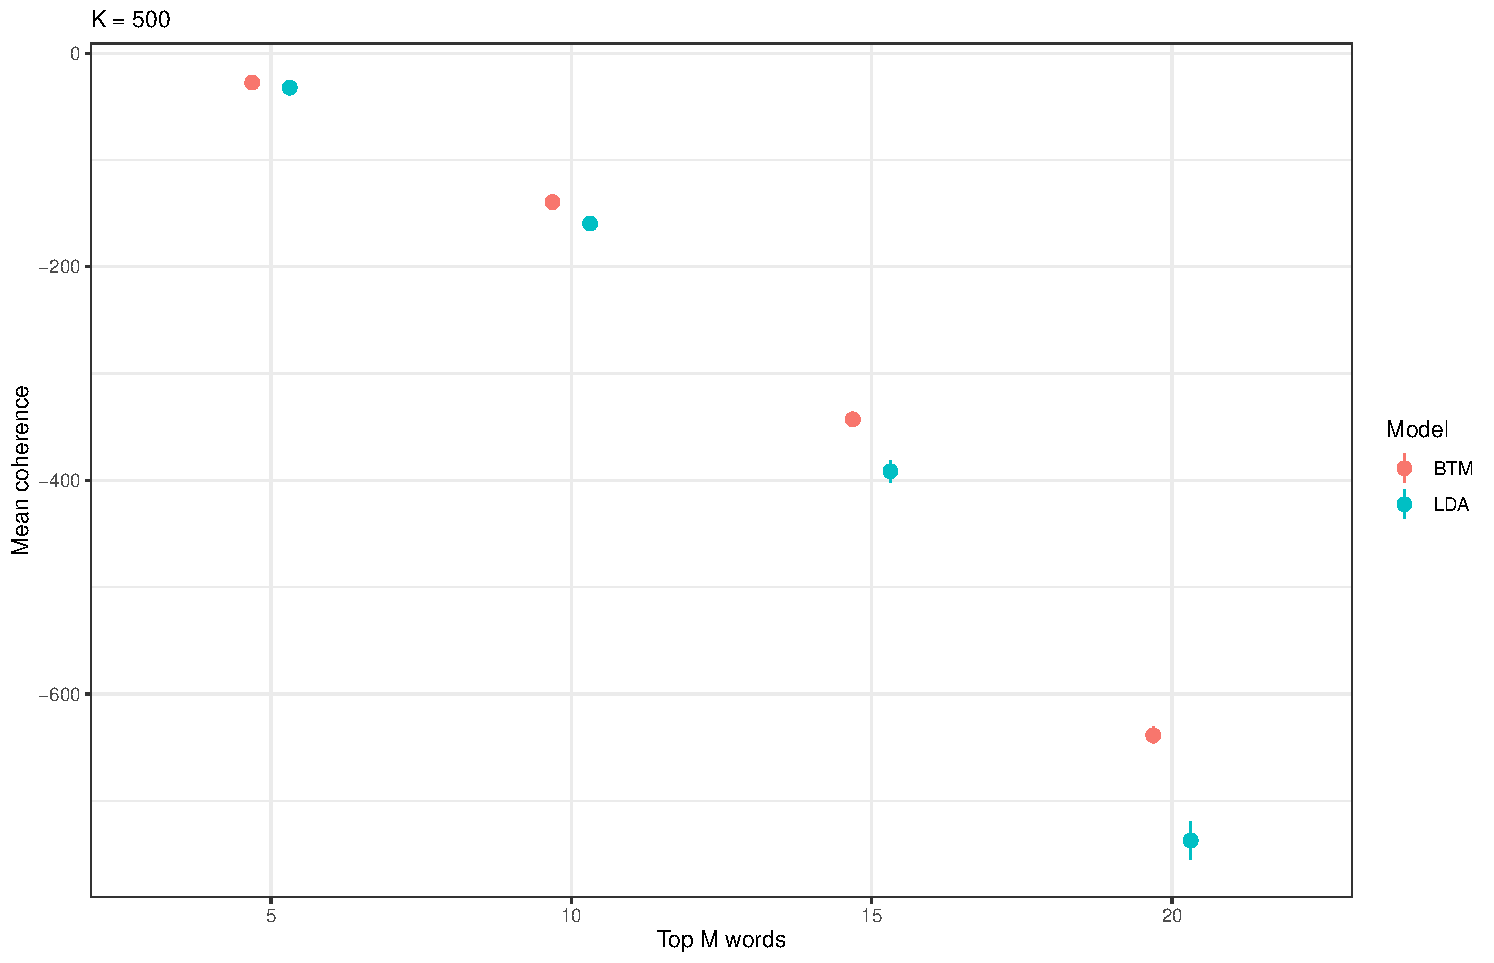
\includegraphics[width=\linewidth]{coherence_k500}
	\caption{\label{fig:coherence}This caption explains the above plot.}
\end{figure}

\lipsum[5]
Looking at the figure above (\autoref{fig:coherence}), I don't remember what I was going to say.


\section{Second section}

\lipsum[6-7]

\section{Third section}

Everything I do is in R 4.0\citep{R-4.0.0}. \ttt{purrr}\citep{purrr} is a great package. I also used a
bunch of other packages\citep{qs,dplyr,ggplot2}.


\clearpage

\chapter{Data preparation}

\section{First section}

\lipsum[8-9]

\section{Second section}

\lipsum[10-11]

\clearpage

\newgeometry{margin=0.7in}

\begin{landscape}

\begin{table}
\centering
\resizebox{\linewidth}{!}{%
\begin{tabular}{lllllll}
\toprule
\ttt{user\_id}
& \ttt{status\_id}
& \ttt{created\_at}
& \ttt{text}
& \ttt{is\_retweet}
& \ttt{hashtags}
& \ttt{lang}\\
\toprule
%
833499844517961728 
& 1255290686250811392 
& 2020-04-29 00:19:56
& \pbox{8cm}{The NY Dem Presidential Primary on\\ 6/23 is canceled due to COVID-19. Other elections on 6/23 will still take place:\\ https://t.co/0P6PMPq20h\\ - Rock the Vote}
& \ttt{FALSE}
& \ttt{NA}
& en\\
\midrule
581180392 
& 1254511313331597314 
& 2020-04-26 20:42:59
& \pbox{8cm}{In the midst of the current \#pandemic, it is more important than ever to get creative\\ with your \#homeworkout. One great\\ \#trainfromhome option includes making a sandbag from a laundry bag. Here's how to implement sandbag circuits:\\ https://t.co/Ottxy2YZAq}
& \ttt{FALSE}
& \pbox{6cm}{\ttt{"pandemic",}\\ \ttt{"homeworkout",}\\ \ttt{"trainfromhome"}}
& en\\
\midrule
819296296062201857
& 1304087649011953665
& 2020-09-10 16:01:38
& \pbox{8cm}{\#Masks serve 2 purposes:\\[3mm] 1) To remind everyone that there is supposed to be a deadly pandemic, despite nobody knowing anybody who is sick with covid, and \\[3mm] 2) To increase incidence of pulmonary illnesses, which will later be blamed on covid. Proof: See my pinned tweet.}
& \ttt{FALSE}
& \ttt{"Masks"}
& en\\
\midrule
2350488460 
& 1322387795718119425
& 2020-10-31 03:59:53
& \pbox{8cm}{\#GOPBetrayedAmerica decisions are being made to take your voice/vote away. The same \#GOPCorruptionOverCountry that\\ won't respond with help for every American\\ during this once a century pandemic\\ https://t.co/Gg5gecx7tb}
& \ttt{FALSE}
& \pbox{6cm}{\ttt{"GOPBetrayedAmerica",}\\ \ttt{"GOPCorruptionOverCountry"}}
& en\\
\bottomrule
\end{tabular}}
\caption{\label{tbl:tweetsample}This caption describes the above table.}
\end{table}

\end{landscape}

\clearpage

\restoregeometry

\section{Third section}

\lipsum[12-13]

Did you see \autoref{tbl:tweetsample}?


\clearpage

\bibliographystyle{unsrtnat}
\bibliography{bibliography}

\label{endmainmatter} % For automatic counting of pages

\end{document}
